\documentclass{school-22.211-notes}
\date{May  9, 2012}

\begin{document}
\maketitle

\lecture{Reconstruction/De-homogenization Methods}
In this lecture we consider given a homogenized solution, how to we re-construct the heterogeneous solution. Three references: Scott Palmtag's MIT PhD thesis `Advanced Nodal Methods for MOX Fuel Analysis' for good detailed math, Ken Rempse' NSE paper `SIMULATE-3 Pin Power Reconstruction: Methology and Benchmarking,' Qunlei Jiang's NCS MS thesis for detailed plots of complex terms `Intra-nodal Study for the Mixed LEU-MOX Cores.' 

\topic{Superposition Assumptions}
Basically we assume that the detailed flux distribution can be approximated by superposition of homogeneous nodal fluxes and lattice fluxes. That is, 
\eqn{ \phi_g^{het} (x,y) &= \phi_g^{hom}(x,y) \phi_g^{SA} (x,y) }
Keep in mind that, as the example in Fig.~\ref{dehom-supercomposing}, the heterogeneous flux should be continuous acorss the material boundary now, 
\eqn{\left. \phi_g^{SA, UO2} (x)  \phi_g^{hom, UO2} (x) \right|_{x=0} = \left. \phi_g^{SA, MOX} (x)  \phi_g^{hom, MOX} (x) \right|_{x=0} }
\begin{figure}[ht]
  \centering
  \includegraphics[width=4in]{images/methd/dehom-supercomposing.png}
  \caption{Supercomposing Thermal Flux in a 1D UO2/MOX problem} \label{dehom-supercomposing}
\end{figure}
In a similar fashion, we can superposition the pin power as well, in which case would need to know the pin-wise fission cross section form functions as well as the group-wise flux form functions. This would be a lot of data considering that form function, like cross sections and discontinuity factors have to be built into giant libraries vs. burnup, temperature, density etc). 

Consequently, most often powers are reconstructed be approximated by a superposition of homogeneous nodal powers and lattice pin powers. 
\eqn{ P^{het} (x,y) = P^{hom} (x,y) P^{SA} (x,y) }
where
\eqn{ P^{hom} (x,y) = \Sigma_{f1}^{hom} (x,y) \phi_1^{hom} (x,y) + \Sigma_{f2}^{hom} (x,y) \phi_2^{hom} (x,y) }
For detailed pin power reconstruction, one needs 2D $(x,y)$ shapes of fluxes -- which are not directly available. Nodal methods only provide flux shape information for the 1D shape in each direction. Cross section shapes are also only 1D averages. 


\clearpage
\topic{Non-Separable Flux Expansion}
\begin{enumerate}
\item We asume nodal solution is known and construct a non-separable flux expansion for each group, analogous to the 1D SANM expansions as the following:
\begin{figure}[ht]
  \centering
  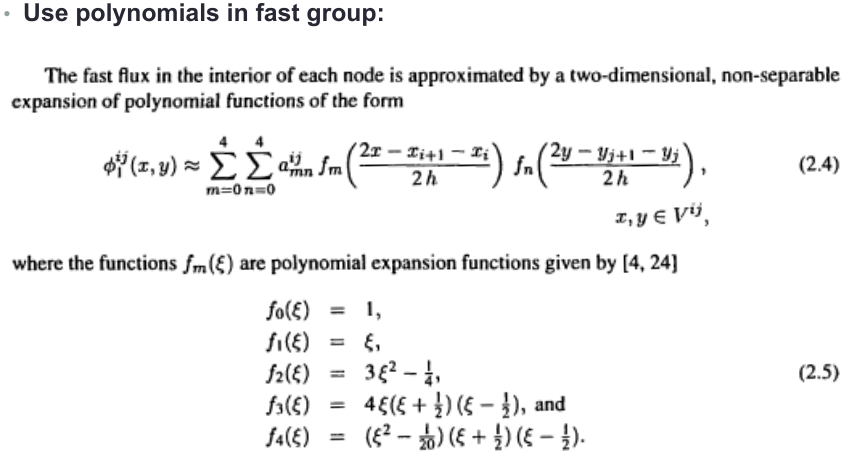
\includegraphics[width=5in]{images/methd/dehom-fast.png} 
  \\
  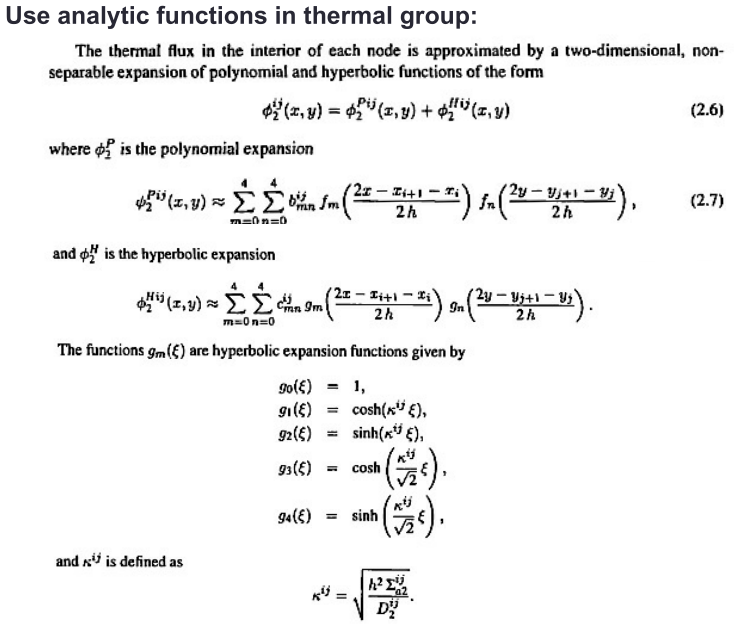
\includegraphics[width=5in]{images/methd/dehom-thermal.png}   
  \caption{Non-Separable Flux Expansion} \label{dehom-energy-group}
\end{figure}

\item Using 5th order polynomial, there are 25 unknown coefficients in the fast group ($a_{mn}$, where $m,n$ each goes from $0$ to $4$). For the thermal group, because of the polonomial and the hyperbolic functions, there appear to be 50 unknowns $b_{mn}, c_{mn}$; but it is really 25, because the other 25 for the specific colution can be solved from the fast group.

\item We have 9 constrains provided by the nodal solution, 
  \begin{itemize}
    \item 1 node average flux per group; 
    \item 4 surface-averaged fluxes per group;
    \item 4 surface-averaged net currents per group. 
  \end{itemize}
  
\item To supplement, the four corner point flux conditions are often used using the KWU method (non-iterative, second-order accurate): 
  \begin{itemize}
    \item Assume fluxes have quadratic shape on each node surface;
    \item Constrain average surface value to be the known nodal surface-averaged flux;
    \item Demand continuity of current in x-direction at the corner point; 
    \item Demand continuity of current in y-direction at the corner point;
    \item Perform post-nodal iteration to simultaneously determine all corner point fluxes;
  \end{itemize}

\item For each energy group, we have $9 + 4 = 13$ constrains and 25 unknowns. What we do is that we disregard the 12 highest order cross terms. 
\end{enumerate}

\clearpage
\topic{Corner Point Constraints}
Nodal corner-point fluxes are approximated by assuming that intra-nodal flux distributions are separable: 
\eqn{ \phi_{g,i,j}(x,y) = \frac{\phi_{g,i,j} (x) \phi_{g,i,j} (y)}{\bar{\phi}_{g,i,j}} }
Since the expansion has been performed about the corner point, the error in each estimator of the corner-point flux can be determined to be second-order; for instance, one of the corners has an error like, 
\eqn{ \epsilon = \frac{1}{4 \phi_{cp}} \frac{\partial \phi}{\partial x} \frac{\partial \phi}{\py} - \frac{1}{4} \frac{\partial^2 \phi}{\px \py} + O \left( \frac{\partial^3 \phi}{\partial^3 u} \right) }
Another important point is that the \textit{heterogeneous corner point flux has to be continuous}. Thus we need corner point ratios that are analogous to discontinuity factors that can be edited from lattice calculations. 
\begin{itemize}
\item In the general case, the corner-point fluxes are determined by averaging the four estimates of the heterogeneous corner-point flux, $cp$ is corner point, 
  \eqn{ \phi_g^{het,cp} &= \frac{1}{4} \left[ \phi_{g,i,j}^{hom,cp} \phi_{g,i,j}^{fct,cp} + \phi_{g,i+1,j}^{hom,cp} \phi_{g,i+1,j}^{fct,cp} + \phi_{g,i,j+1}^{hom,cp} \phi_{g,i,j+1}^{fct,cp} + \phi_{g,i+1,j+1}^{hom,cp} \phi_{g,i+1,j+1}^{fct,cp} \right] }

\item In order to satisfy the continuity conditions of reconstructed fluxes, the best-estimate homogeneous corner-point fluxes for each node are computed by, 
  \eqn{ \hat{\phi}_{g,i,j}^{hom,cp} = \frac{\phi_g^{het,cp}}{\phi_{g,i,j}^{fct,cp}} }
  The reconstructed corner point fluxes are then continuous. \textit{CP ratio is the corner point analogue of ADF for assembly edges.}
\end{itemize}
Surface constrains preserve flux shape. Each corner has 4 surfaces connected to it. 


\clearpage
\topic{Basic Reconstruction Steps}
\begin{enumerate}
\item Solve normal nodal model global equations.
\item Determine corner point fluxes. 
\item Compute 2D fluxe expansions coefficients. 
\item Compute 2D fission cross section shapes.
\item Integrate flux shape times cross section shape over each pin cell location to get `homogenized' pin powers. 
\item Evaluate lattice `pin power form function' at the nodal exposure. 
\item Multiply homogenized pin power by the pin power form function to get the `heterogeneous' pin powers.
\item Integrate the heterogeneous pin powers over time (usually exposure) to get heterogeneous pin burnups. 
\item Determine pin-wise thermal margins (DNBR, CPR, LHGR, etc). 
\end{enumerate}




\clearpage
\topic{Homogeneous Cross Section Shape}
The reconstructed pin powers have errors. The first thing we want to check is the 2 group cross sections, which turn out to be only approximately correct as in Fig.~\ref{dehom-2g-err}. Errors arise from spatially constant cross section approximation, not from inadequancies of the spatial flux representations. 
\begin{figure}[ht]
  \centering
  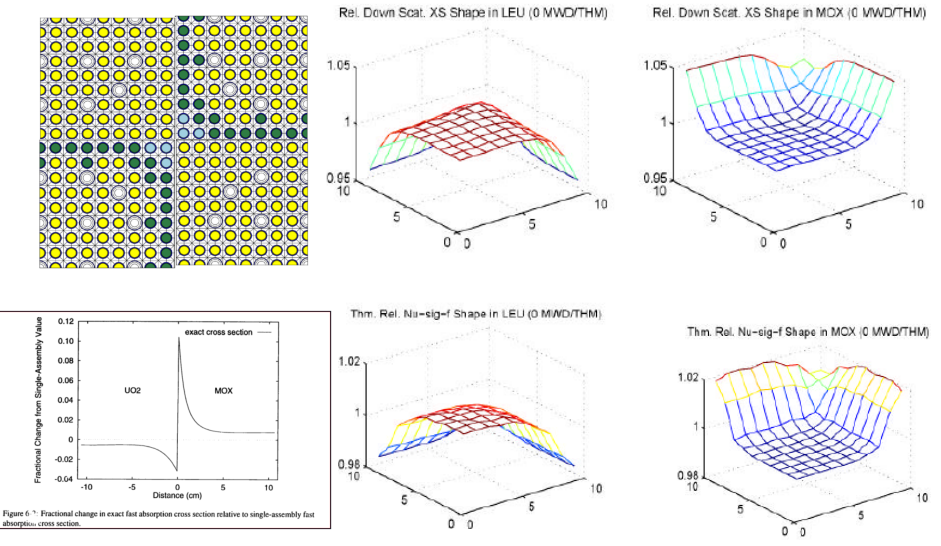
\includegraphics[width=5in]{images/methd/dehom-2gxs.png}
  \\
  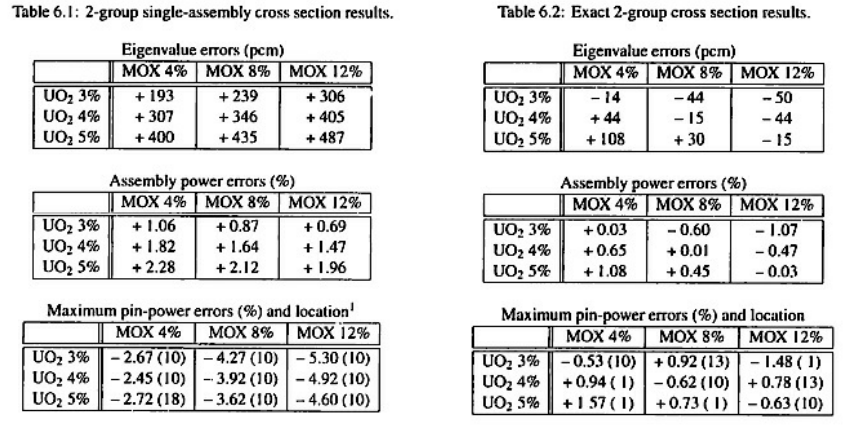
\includegraphics[width=5in]{images/methd/dehom-2gxs-err.png}
  \caption{2 Group Cross Section Errors} \label{dehom-2g-err}
\end{figure}
To adjust the cross sections, we use \hi{instantaneous leakage and spectral corrections}, where SA means single assembly, 
\eqn{ \frac{\Sigma_{\alpha 1}^B (x) - \Sigma_{\alpha 1}^{SA}}{\Sigma_{\alpha 1}^{SA}} &= B_{\alpha} \left[ \frac{-D_1 \nabla^2 \phi_1(x)}{\Sigma_{a1}(x) \phi_1(x) + \Sigma_{21} (x) \phi_1(x)} \right] } 
\eqn{\frac{\Sigma_{\alpha g}^S(x) - \Sigma_{\alpha g}^B(x)}{\Sigma_{\alpha g}^B(x)} &= \pm C_{\alpha g} \left| \frac{\Gamma(x) -\Gamma^{SA}}{\Gamma^{SA}} \right|^{P_{\alpha g}}  }
where $\Gamma(x) = \frac{\phi_2(x)}{\phi_1(x)}$. As in Fig.~\ref{approx-xs}, we can see the cross section after approximation corrections. 
\begin{figure}[ht]
  \centering
  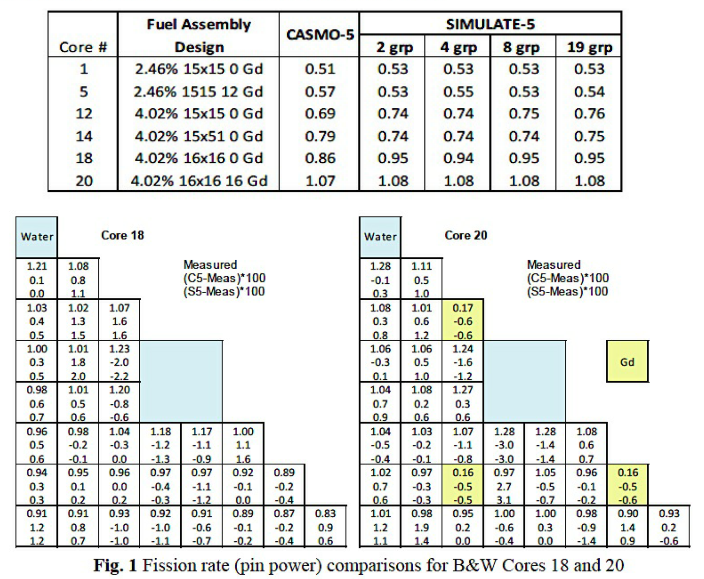
\includegraphics[width=5in]{images/methd/approx-xs.png}
  \caption{Approximate Cross Section Corrections vs. More Groups} \label{approx-xs}
\end{figure}
To measure power of a core, we pull out individual pins and measure the gamma deposited in it to get the power profile of it. The uncertainty comes out to be about 1.5\%, which is considered to be high precision. 

Advanced topic: fixing Cross-sections On The Fly/`Adhop' Method. 

This method is somewhat an empiracle one; hence it is not very robust. Nowadays, nodal methods just go to higher order of energy groups. 

\clearpage
\topic{Nodal Method Summary}
Basically a production-grade nodal code must have, 
\begin{itemize}
\item Accurate lattice data;
\item Coupling to an accurate thermal-hydraulic model;
\item Accurate nodal flux model;
\item Accurate re-homogenization model for cross section heterogeneity;
\item Accurate spatial cross section (homogenized) representation;
\item Accurate non-separable flux (homogenized) model;
\item Accurate pin power form functions;
\item Accumulated pin exposure models. 
\end{itemize}


\lecture{Adjoint Fluxes}
The general idea of adjoint problem is that we can get a pretty accurate prediction of reactivity without knowning $\delta \psi$. There is no reactivity associated with a space and a time (it has a reactivity contribution). Reactivity is always integrated over the entier system because of the denominator. 

\topic{Adjoint Fluxes for Critical Reactor Systems}
We express the transport of diffusion equation in operator notation, 
\eqn{ A\psi &= \frac{1}{k} M \psi &A^*\psi^* &= \frac{1}{k^*} M^* \psi^*  }
We multiply the forward equation by adjoint flux, multiply the adjoint equation by real flux, subtract the two and integrate over the phase space to get, 
\eqn{ \expect{ \psi^*, A\psi}  - \expect{\psi, A^* \psi^*} - \frac{1}{k} \expect{ \psi^*, M \psi} + \frac{1}{k^*} \expect{ \psi, M^* \psi^*} &= 0 }
But recalling the definition of the adjoint operating on any operator $f$, 
\eqn{ \expect{ \psi^*, f\psi} &= \expect{\psi, f^* \psi^*} }
Consequently, 
\eqn{ \expect{ \frac{1}{k} - \frac{1}{k^*} } \expect{ \psi^*, M \psi} &= 0 }
The fundamental mode solution, which is the one we are interested in, has everywhere positive real and adjoint fluxes, and since the fission operator is an everywhere positive operator, we find that the real and adjoint eigenvalus must be identical,
\eqn{ k^* &= k }

\clearpage
\topic{Perturbation Theory Expression for Reactivity}
\begin{enumerate}
\item Again we start from the operator forms, 
\eqn{ A \psi &= \frac{1}{k} M \psi &A^*\psi^* &= \frac{1}{k^*} M^* \psi^*  }
We perturb the operators such that, 
\eqn{ A^* &= A + \delta A   &M^*&=M + \delta M  &\psi^*&=\psi + \delta \psi }
Then the perturbed system using expanded operators becomes, 
\eqn{ (A + \delta A) (\psi + \delta \psi) - \frac{1}{k+\delta k} (M + \delta M) (\psi + \delta \psi) &=0 \label{perturbed-sys}}

\item We expand the $\keff$ term, 
\eqn{ \frac{1}{k+\delta k} = \frac{1}{k} \frac{1}{1 + \delta k /k} = \frac{1}{k} - \frac{\delta k}{k^2} + O(\delta k^2)  }
Plug back into Eq.~\ref{perturbed-sys}, 
\begin{align}
(A + \delta A) (\psi + \delta \psi) &= \frac{1}{k+\delta k} (M + \delta M) (\psi + \delta \psi) \\
(A + \delta A) (\psi + \delta \psi) &= \left( \frac{1}{k} - \frac{\delta k}{k^2}  \right) (M + \delta M) (\psi + \delta \psi) \\
A \psi + A \delta \psi + \delta A \psi &= \frac{1}{k} M \psi + \frac{1}{k} M \delta \psi + \frac{1}{k} \delta M \psi - \frac{\delta k}{k^2} M \psi + O(\delta^2)  
\end{align}
\eqn{ \overbrace{ \left( A - \frac{1}{k} M \right) \psi}^{\to 0} + \left( A - \frac{1}{k} M \right) \delta \psi + \left( \delta A - \frac{1}{k} \delta M \right) \psi &= - \frac{\delta k}{k^2} M \psi + O(\delta^2)  }
\eqn{ -\frac{\delta k}{k^2} M \psi &= \left( \delta A - \frac{1}{k} \delta M \right) \psi + \left( A - \frac{1}{k} M \right) \delta \psi + O (\delta^2) }
Multiply by $\psi^*$ and integrating over phase space, 
\eqn{ - \frac{\delta k}{k^2} \expect{ \psi^*, M \psi} &= \expect{ \psi^*, \left( \delta A - \frac{1}{k} \delta M \right) \psi } + \overbrace{ \expect{\psi^*, \left( A - \frac{1}{k} M \right) \delta \psi} }^{\textcircled{1}} + O(\delta^2) \label{perturbed-sys2} }

\item First-order perturbation theory: we use the definition of adjoint operator for any operator, 
\eqn{ \textcircled{1} =  \expect{\psi^*, \left( A - \frac{1}{k} M \right) \delta \psi} =  \expect{\delta \psi, \left( A^* - \frac{1}{k^*} M^* \right) \psi^*} = 0 }
because $\left( A^* - \frac{1}{k^*} M^* \right) \psi^* = 0$. Then Eq.~\ref{perturbed-sys2} becomes, 
\eqn{ - \frac{\delta k}{k^2} &= \frac{\expect{ \psi^*, \left( \delta A - \frac{1}{k} \delta M \right) \psi }}{\expect{ \psi^*, M \psi} } + O(\delta^2) \label{perturbed-sys3} }
Notice that, 
\begin{itemize}
 \item There are only second order errors in reactivity. 
 \item Notice Eq.~\ref{perturbed-sys3} is clearly much more accurate than our previous expression, which has a first order error in reactivity without knowing $\delta \psi$, 
   \eqn{ - \frac{\delta k}{k^2} &= \frac{ \left(\delta A - \frac{1}{k} \delta M\right) \psi + \left( A - \frac{1}{k} M \right) \delta \psi}{M \psi} + O (\delta^2) }
\end{itemize}

 \item Finally making use of the definition of reactivity, 
   \eqn{ \rho &= \frac{k-1}{k} &\Rightarrow \rho^* - \rho &= \frac{k^* - 1}{k^*} - \frac{k-1}{k} = \frac{\delta k}{k^* k} &\delta \rho &= \frac{\delta k}{k^2} + O(\delta k^2) }
   One obtains the first order perturbation (FOP) expression for reactivity, 
   \eqn{ \boxed{\delta \rho \approx \frac{\expect{\psi^*, \left( \frac{1}{k} \delta M - \delta A \right) \psi }}{\expect{\expect{\psi^*, M \psi}}}  } }
\end{enumerate}
Interpretations of the $\delta \rho$ equation, 
\begin{itemize}
\item One can evaluate reactivity resulting from any changes in operator, e.g., fuel temperature, coolant density, boron concentration, by simply evaluating delta cross sections convoluted on unperturbed real and adjoint fluxes. 

\item Because of the linearility of the first-order perturbation theory, we can super-impose: 
  \begin{itemize}
  \item reactivity contributions from perturbations in different spatial regions;
  \item reactivity effects from perturbations in different phenomenon, e.g., coolant density and temperature. 
  \end{itemize}

\item Each reactivity perturbation can be computed without need for solving for perturbed spatial flux distributions. 
\end{itemize}

\clearpage
\topic{Relating Adjoint Flux to Neutron Population}
Recall from the point kinetics that the neutron population is given by, 
\begin{align}
  \ddt N(t) &= \frac{\rho(t) - \Sum_i \beta_i}{\Gamma} N(t) + \Sum_i \lambda_i C_i(t) + Q \\
  \ddt C_i (t) &= \frac{\beta_i}{\Gamma} N(t) - \lambda_i C_i (t)
\end{align}
For reactivity equals zero, 
\eqn{ \ddt N(t) = Q \Rightarrow N(t) = N_0 + Q(t-t_0)}
Thus neutron polulation grows linearly in time with an external source (Q = neutrons per second). But consider introducing $Q$ neutrons: at time zero at position, energy, and direction $(\vecr, \Omegahat, E)$ then
\eqn{ \ddt N(t) &= Q  \delta (t - t_0) \Rightarrow N(\infty) = N_0 + Q x} 
Or 
\begin{align}
 \ddt N(t) &= Q \delta (t - t_0) \Rightarrow N(\infty) = N_0 + Q \psi^* (\vecr, \Omegahat, E)  \\
 \Aboxed{\frac{N(\infty) - N_0}{Q} &= \psi^* (\vecr, \Omegahat, E)  }
\end{align}
\hi{The adjoint flux is defined as the asymptotic increase in total neutron population of a critical reactor for a neutron introduced a position r, direction omega, and energy E.} The adjoint is only defined for what reaction that we are interested in: in a critical reactor, that is neutron population; in a subcritical system, like the one in detector, then it is whatever purpose, like detector response, that we are interested in. 


\clearpage
\topic{Multi-Group Real and Adjoint Flux Equations}
\begin{align}
- \gradient D_g (\vecr) \gradient \phi_g(\vecr) + \Sigma_{tg} (\vecr) \phi_g(\vecr) &= \chi_g \Sum_{g'=1}^G \nu \Sigma_{fg'} (\vecr) \phi_{g'}(\vecr) + \Sum_{g'=1}^G \Sigma_{sg'\to g} (\vecr) \phi_{g'}(\vecr) \\
 \gradient D_g (\vecr) \gradient \phi_g^* (\vecr) + \Sigma_{tg} (\vecr) \phi_g^* (\vecr) &= \chi_{g'} \Sum_{g'=1}^G \nu \Sigma_{fg} (\vecr) \phi_{g'}^* (\vecr) + \Sum_{g'=1}^G \Sigma_{sg\to g'} (\vecr) \phi_{g'}^*(\vecr)
\end{align}
For two group, infinite medium case, with effective downscatter only, 
\begin{align}
\left[ \begin{array}{cc}
\Sigma_{a1} + \Sigma_{12} - \frac{1}{\kinf} \nu \Sigma_{f1} & - \frac{1}{\kinf} \nu \Sigma_{f2} \\
- \Sigma_{12} & \Sigma_{a2} \end{array} \right] 
\left[ \begin{array}{c}
\phi_1 \\ \phi_2 \end{array} \right] &= 0  
&\frac{\phi_2}{\phi_1} &= \frac{\Sigma_{12}}{\Sigma_{a2}}  
&\kinf &= \frac{\nu \Sigma_{f1} \phi_1 + \nu \Sigma_{f2} \frac{\Sigma_{12}}{\Sigma_{a2}} }{\Sigma_{a1} + \Sigma_{12}}   \\
\left[ \begin{array}{cc}
\Sigma_{a1} + \Sigma_{12} - \frac{1}{\kinf^*} \nu \Sigma_{f1} & - \Sigma_{12} \\
- \frac{1}{\kinf^*} \nu \Sigma_{f2} & \Sigma_{a2} \end{array} \right] 
\left[ \begin{array}{c}
\phi_1^* \\ \phi_2^* \end{array} \right] &= 0  
&\frac{\phi_2^*}{\phi_1^*} &= \frac{\frac{1}{\kinf^*} \nu \Sigma_{f2}}{\Sigma_{a2}}  
&\kinf^* &= \frac{\nu \Sigma_{f1} \phi_1 + \nu \Sigma_{f2} \frac{\Sigma_{12}}{\Sigma_{a2}} }{\Sigma_{a1} + \Sigma_{12}} 
\end{align}
The above expressions show that knowing cross sections, we know $\kinf$, hence we know $\kinf^* = \kinf$, then we can solve for $\frac{\phi_2^*}{\phi_1^*}$. 
\end{document}

\begin{figure}[ht]
  \centering
  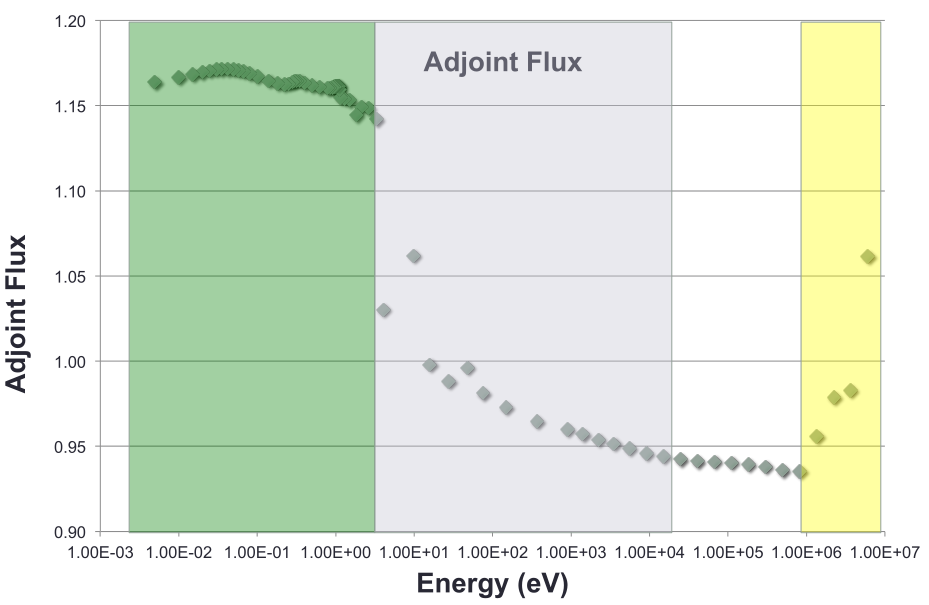
\includegraphics[width=5in]{images/methd/adjoint-spec.png}
  \caption{PWR Lattice Adjoint Spectrum}
\end{figure}

\begin{figure}[ht]
  \centering
  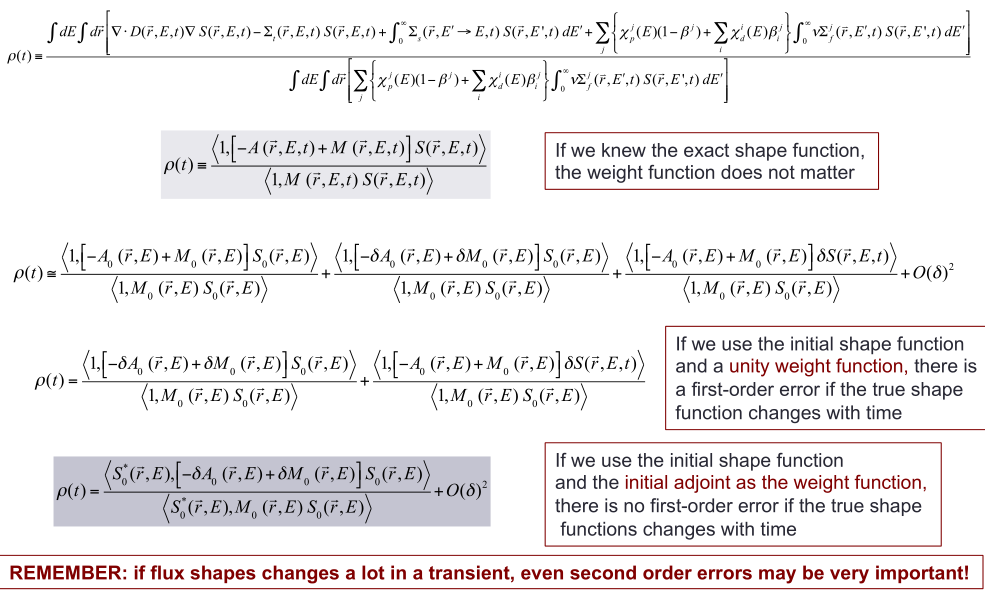
\includegraphics[width=5in]{images/methd/adjoint-weighted-reactivity.png}
  \\
  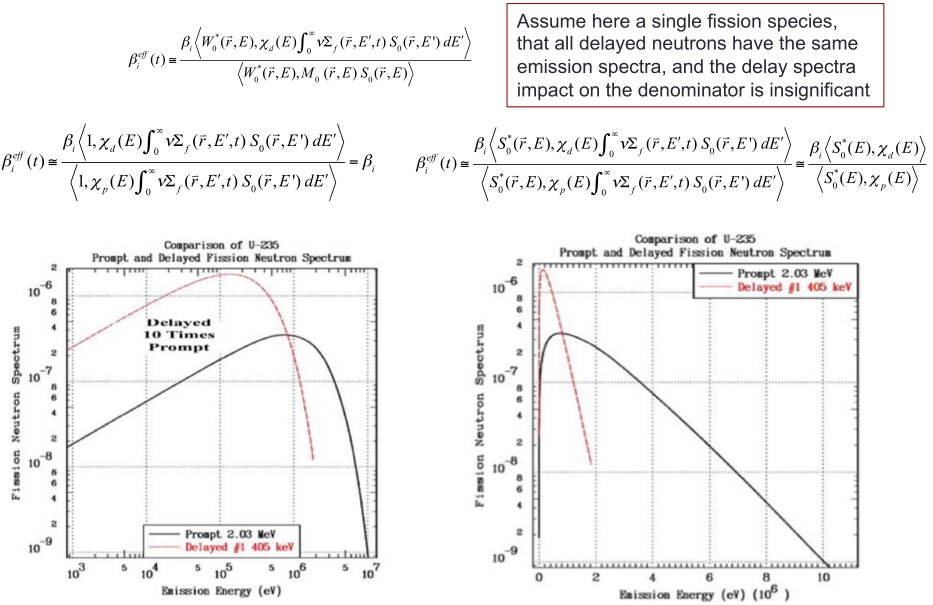
\includegraphics[width=5in]{images/methd/adjoint-weighted-reactivity-2.png}
  \caption{Adjoint Weighted Reactivity}
\end{figure}

\begin{figure}[ht]
  \centering
  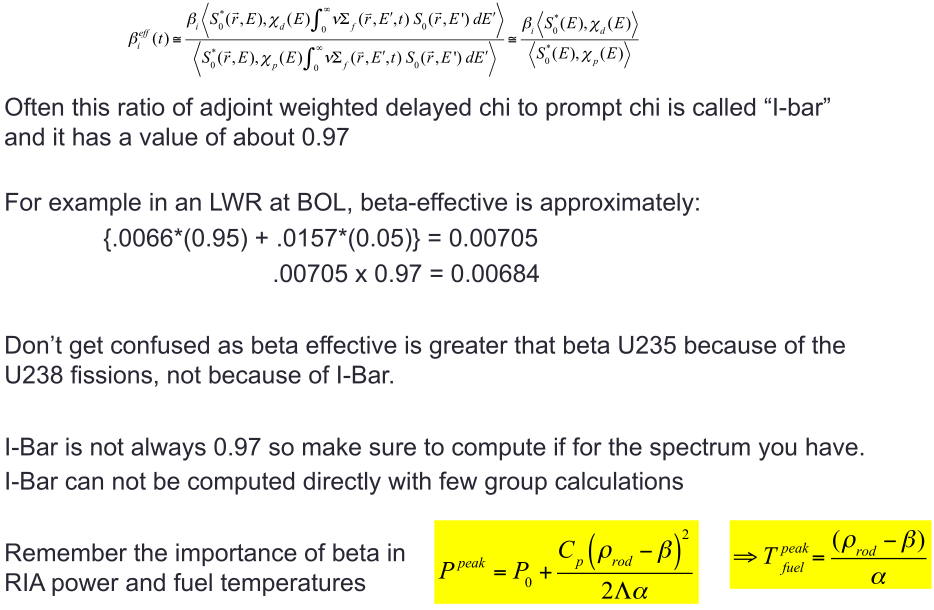
\includegraphics[width=5in]{images/methd/beta-effective.png}
  \caption{LWR Beta Effective}
\end{figure}
